% ============================================================
% main.tex  ---  AMPS: An Anticipatory Multi-Agent Framework for
% Energy-Efficient Pump Scheduling under Pilgrimage-Driven Demand Surges
% Target venue: Arabian Journal for Science and Engineering (Springer)
%
% NOTE ON TEMPLATE: This file uses the standard `article` class so it
% compiles in any environment. For AJSE submission, replace the preamble
% with Springer's official class:  \documentclass[sn-mathphys]{sn-jnl}
% (download from the journal's submission-guidelines page) and move the
% abstract/keywords into the Springer macros. Section content is unchanged.
%
% STATUS: Abstract, Introduction, Related Work, and Problem Formulation are
% fully drafted. Framework (Sec. 4) is scaffolded with the design already
% agreed. Results (Sec. 6) intentionally contains NO numbers yet -- those
% are produced by the simulation runs. No placeholder results appear in
% any results table (per the citation/integrity rules).
% ============================================================

\documentclass[11pt,a4paper]{article}

\usepackage[utf8]{inputenc}
\usepackage[T1]{fontenc}
\usepackage{times}
\usepackage[margin=1in]{geometry}
\usepackage{amsmath,amssymb}
\usepackage{graphicx}
\usepackage{booktabs}
\usepackage{placeins}
\usepackage{tabularx}
\newcolumntype{Y}{>{\raggedright\arraybackslash}X}
\newcolumntype{R}{>{\raggedleft\arraybackslash}X}
\usepackage{hyperref}
\usepackage[numbers,square]{natbib}
\usepackage{xcolor}
% Render multiple citations as [1][2] (separate brackets), not [1, 2]:
\makeatletter
\def\NAT@open{[}
\def\NAT@close{]}
\def\NAT@sep{][}
\makeatother
\usepackage{url}
\usepackage{float}
\usepackage{tikz}
\usetikzlibrary{arrows.meta,positioning,fit,backgrounds}
\usepackage[ruled,vlined]{algorithm2e}

\bibliographystyle{unsrtnat}

\title{\textbf{AMPS: An Anticipatory Multi-Agent Framework for Pump Scheduling
under Predictable Demand Surges}}

\author{
Hamzah Faraj\,$^{1}$\thanks{Corresponding author: \texttt{f.hamzah@t.edu.sa}}
\quad Abdullah H. Alshahri\,$^{2}$
\quad Mohamed S. Soliman\,$^{3}$ \\[4pt]
\small $^{1}$ Department of Science and Technology, Ranyah College, Taif University, Taif 21944, Saudi Arabia \\
\small $^{2}$ Department of Civil Engineering, Faculty of Engineering, Taif University, P.O.\ Box 11099, Taif 21974, Saudi Arabia \\
\small $^{3}$ Department of Electrical Engineering, College of Engineering, Taif University, Taif 21944, Saudi Arabia \\[2pt]
\small \texttt{f.hamzah@t.edu.sa} \quad \texttt{aalshahri@tu.edu.sa} \quad \texttt{soliman@tu.edu.sa}}

\date{}

\begin{document}
\maketitle

% ============================================================
\begin{abstract}
\noindent
Pumping is the largest controllable energy expenditure in water distribution
networks, and its scheduling becomes acute where demand is subject to large,
recurring, calendar-driven surges. Such surges arise in many contexts---major
sporting events, tourist-season peaks, and most prominently the Saudi Hajj and
year-round Umrah pilgrimages, where daily pumping to Makkah and the holy sites
averages roughly 750{,}000~m\textsuperscript{3} and exceeds
1{,}000{,}000~m\textsuperscript{3} on peak days, a swing that conventional
rule-based and metaheuristic schedules handle poorly. Existing learning-based
controllers are typically single-task and reactive, are benchmarked under
heterogeneous setups that frustrate fair comparison, and do not exploit the fact
that such surges are predictable in timing. This paper proposes AMPS, an
anticipatory multi-agent framework that integrates three stages: a
calendar-aware demand forecaster, a cooperative multi-agent reinforcement
learning controller in which the number of agents is derived from network
coupling structure, and a physics-based feasibility layer that enforces
hydraulic and supply constraints within the simulation. The framework is general
and network-agnostic; the Hajj/Umrah pilgrimage is used as the flagship numeric
case study because it is the largest documented predictable surge in the world.
AMPS is evaluated entirely in simulation on public benchmark networks (US, UK,
and international competition origins) using the EPANET hydraulic engine, with
the pilgrimage surge ratio used as one illustrative scenario parameter alongside
a sensitivity sweep across event-type magnitudes. Against rule-based and
optimization baselines re-implemented in the same environment, AMPS is assessed
on pumping energy, energy cost, demand satisfaction, and pump switching. The
framework's adaptive multi-agent decomposition consistently matches or exceeds a
centralized optimizer, yielding energy reductions of up to $16.7\%$ at held
demand satisfaction on an international benchmark network, while the simulation
environment is validated to conserve mass to within $\sim\!10^{-4}\%$.
The framework and its transferable principle---anticipatory multi-agent control
under predictable demand surges---are intended to generalize beyond water to
other infrastructure systems facing scheduled load spikes.
\\[6pt]
\textit{Keywords}: pump scheduling; multi-agent reinforcement learning; water
distribution networks; anticipatory control; energy efficiency; demand
forecasting; predictable demand surges; EPANET
\end{abstract}

% ============================================================
\section{Introduction}
\label{sec:intro}

Drinking-water utilities are among the most energy-intensive public services,
and within a typical water distribution network (WDN) the energy consumed by
pumping dominates controllable operating cost. Because pumps must lift and
pressurize water against both elevation and demand, the timing of their
operation---how much is pumped, when, and through which station---directly
determines both the electricity bill and the reliability of supply. Improving
pump scheduling therefore offers one of the largest available levers for
reducing the energy footprint of urban water systems without any change to
physical infrastructure.

The problem becomes considerably harder when demand is not merely variable but
subject to large, \emph{predictable} surges. Many water systems experience such
surges---seasonal tourism, major scheduled events, and religious
gatherings---in which demand rises sharply over short, calendar-determined
periods. The most extreme instance anywhere in the world, and the flagship case
study of this paper, is the Saudi pilgrimage cycle. During the annual Hajj, and
throughout the year during Umrah, the populations of Makkah and Madinah rise by
millions over short, well-defined periods. The scale of the resulting water
operation is documented by the national water agencies: daily pumping to Makkah
and the holy sites of Mina, Arafat, and Muzdalifah averages on the order of
750{,}000~m\textsuperscript{3} and exceeds one million m\textsuperscript{3} on
Arafat Day and during Eid, supported by operational and strategic storage in
excess of 3.2~million m\textsuperscript{3} \citep{SWA2025HajjReadiness}. Supply
originates at desalination plants along the western coast and is conveyed to the
holy sites through long strategic transmission systems and large reservoirs
\citep{NWC2025Madinah}. Two features make this an exacting control problem: the
surge is severe in magnitude, and the water must frequently be lifted across
significant elevation, so that pumping energy is sensitive to both load and head
simultaneously. Crucially, across all of these settings the \emph{timing} of the
surge is known in advance---a structural property that conventional schedules do
not exploit.

Conventional approaches to pump scheduling fall into two families, each with a
characteristic weakness under these conditions. Rule-based schedules driven by
tank-level triggers are simple and robust but cannot anticipate or economically
absorb a large surge. Metaheuristic optimization (for example genetic
algorithms) can produce high-quality schedules but requires many hydraulic
evaluations, which makes real-time use under changing demand computationally
expensive \citep{Hu2023EPPO}. Deep reinforcement learning (DRL) has recently been
shown to address the latter limitation by shifting the heavy computation to an
offline training phase: once trained, an agent maps the observed network state
to a pumping decision in milliseconds, and reported energy or cost savings are
competitive with optimization while remaining far faster at runtime
\citep{Hu2023EPPO,Pei2025RTPump}. Multi-agent formulations extend this idea to
the coordination of several pumps or valves \citep{Hu2023MARL}.

Despite this progress, three gaps remain. First, the majority of DRL controllers
are \emph{single-task and reactive}: they respond to demand only after it
changes, even when the surge is known in advance from a fixed calendar---as is
the case for recurring scheduled events including major sporting tournaments,
mass gatherings, and seasonal-tourism peaks. Second, reported results are
produced under \emph{heterogeneous experimental setups} (different networks,
baselines, and demand profiles), which makes cross-study comparison unreliable
and obscures how much of a reported gain is attributable to the method as
opposed to the test case. Third, no \emph{reproducible, public-benchmark} study
evaluates surge-resilient scheduling across the heterogeneous conditions---load,
temperature, elevation, and tariff---that characterize the regions where such
events recur.

This paper addresses these gaps with a framework we call AMPS (Anticipatory
Multi-agent Pump Scheduling). The contributions are:

\begin{enumerate}
  \item \textbf{The AMPS framework}: a generalizable, three-stage architecture
  that integrates calendar-aware demand forecasting, cooperative multi-agent
  reinforcement learning control, and a physics-based feasibility layer, so that
  predictable surges are anticipated rather than merely absorbed
  (Section~\ref{sec:framework}).
  \item \textbf{A reproducible surge case-study suite} built on public benchmark
  networks and parameterized by load, temperature, elevation, and time-of-use
  tariff, with the Hajj and Umrah pilgrimage as the flagship case alongside
  global surge regimes, released as an independently reusable artifact
  (Section~\ref{sec:expdesign}).
  \item \textbf{A controlled, single-environment benchmarking protocol} in which
  rule-based, optimization, and single-agent learning baselines are
  re-implemented and evaluated under identical conditions, enabling a fair
  comparison (Section~\ref{sec:expdesign}).
  \item \textbf{An ablation} that isolates the contribution of each framework
  stage, complemented by sensitivity and scalability analyses
  (Section~\ref{sec:results}).
  \item \textbf{Empirical evidence of generalization} across both Saudi and
  global cities under heterogeneous conditions (load, temperature, elevation,
  tariff), \emph{benchmarked against published results on shared public
  networks}, with validation of the simulation and forecasting components and an
  open-source release of code and configurations
  (Sections~\ref{sec:results}--\ref{sec:discussion}).
\end{enumerate}

The remainder of this paper is organized as follows.
Section~\ref{sec:related} reviews related work on optimization-based and
learning-based pump scheduling, multi-agent and physics-informed control, demand
forecasting, and regional water systems, and states the research gap.
Section~\ref{sec:problem} formulates the pump-scheduling problem and the
associated decision process.
Section~\ref{sec:framework} presents the AMPS framework.
Section~\ref{sec:expdesign} details the experimental design, including the
network, the scenario suite, baselines, metrics, and the reproducibility
protocol.
Section~\ref{sec:results} reports the results, including the main comparison,
the surge and generalization analyses, and the ablation.
Section~\ref{sec:discussion} discusses the findings and their implications,
Section~\ref{sec:limitations} states the limitations, and
Section~\ref{sec:conclusion} concludes.

% ============================================================
\section{Related Work}
\label{sec:related}

\subsection{Optimization-based pump scheduling}
The classical formulation of pump scheduling seeks the pump operations that
minimize energy cost over a horizon subject to hydraulic and service
constraints. Metaheuristic search---genetic algorithms and related
population-based methods---has long been the workhorse for this nonlinear,
constrained problem because it copes with the discrete on/off structure of pump
operation and with the nonconvex hydraulics. Its decisive limitation for
operational use is computational: each candidate schedule must be evaluated
through a full hydraulic simulation, and the large number of evaluations
required makes real-time rescheduling under changing demand impractical
\citep{Hu2023EPPO}. Comprehensive reviews of water-distribution system operation
and design catalogue this trade-off across decades of optimization research
\citep{Mala2016WDNoptReview,MalaJetmarova2018Design}, and energy-efficiency
reviews confirm pumping as the dominant controllable cost
\citep{Coelho2014Efficiency}. Genetic-algorithm scheduling remains the canonical
metaheuristic baseline: \citet{Luna2019Energy} report up to $25\%$ energy
reduction through demand- and tariff-aware GA scheduling, while exact approaches
such as branch-and-bound have been explored for smaller systems but scale poorly
\citep{Menke2016BnB}. This bottleneck is the principal motivation for the shift
toward learning-based controllers that move the heavy computation offline.

\subsection{Learning-based control}
Deep reinforcement learning reframes scheduling as a sequential decision process
in which an agent, trained offline, maps the current network state to a pumping
action at negligible runtime cost. \citet{Hu2023EPPO} propose an
exploration-enhanced proximal policy optimization (PPO) scheme that learns
policies for varying demand distributions, reduces energy cost through a
tank-level penalty, and produces decisions in a fraction of a second.
\citet{Pei2025RTPump} train PPO agents for real-time scheduling and compare them
against genetic-algorithm and robust-optimization baselines on benchmark
networks, finding the learned policies competitive on operational cost while more
robust to demand uncertainty. Earlier, \citet{Hajgato2020DRLEPANET} demonstrated
DRL for real-time pump optimization coupled to EPANET, and
\citet{Ledesma2024SafeRL} applied safe RL to water-quality (water-age) control,
reflecting growing attention to constraint satisfaction during learning. Reviews
of RL across water systems \citep{Negm2024RLWaterReview} and in the adjacent
wastewater-treatment domain \citep{Croll2023RLWWTP} document both the promise and
the recurring challenges of start-up safety, sample efficiency, and real-world
deployment. These studies establish that DRL can match
optimization-quality schedules at a runtime suitable for real-time control, but
they share two properties relevant to the present work: the controllers are
trained to react to the observed state rather than to anticipate a known future,
and each is evaluated on its own network and baseline set, so reported savings
are not directly comparable across studies.

\subsection{Multi-agent and constrained control}
Coordinating several pumps---and possibly valves---is naturally a multi-agent
problem, since each actuator influences a shared hydraulic state.
\citet{Hu2023MARL} model pump-and-valve scheduling as a Markov decision process
and apply a multi-agent deep deterministic policy gradient
\citep{Lowe2017MADDPG} to manage demand uncertainty, demonstrating that
decentralized cooperating agents can schedule in real time. Multi-agent methods build on the actor-critic and value-based foundations of
single-agent DRL
\citep{Mnih2015DQN,Lillicrap2016DDPG,Schulman2017PPO,Fujimoto2018TD3,Haarnoja2018SAC},
and are surveyed comprehensively by
\citet{Nguyen2020MARLSurvey,Gronauer2022MADRL,Canese2021MARLReview}; these reviews
identify centralized-training/decentralized-execution (CTDE) as the prevailing
paradigm for cooperative control under partial observability, together with its
central challenges of non-stationarity and credit assignment
\citep{Sutton2018RL}. What
remains underdeveloped is the combination of multi-agent coordination with an
explicit feasibility guarantee and with anticipation of predictable, extreme
surges---precisely the regime that calendar-driven demand events create, of which
the pilgrimage is one well-documented instance.

\subsection{Demand forecasting and anticipation}
Short-term water-demand forecasting is a mature area. Deep recurrent models,
particularly long short-term memory networks \citep{Hochreiter1997LSTM}, have
become the dominant approach: \citet{Guo2018Forecast} established deep learning
for short-term demand, and subsequent work improved accuracy through hybrid and
multivariate designs --- wavelet-decomposition with principal-component analysis
\citep{Pu2023WaveletCNN} and multivariate LSTM incorporating meteorological
inputs \citep{Zanfei2022LSTM} --- as surveyed by \citet{Ghannam2024Review}. A
recurring finding is that calendar and weather covariates materially improve
forecasts of demand peaks. Yet in most scheduling pipelines the forecast and the
controller are treated separately, and the controller ultimately reacts to
realized demand. Where a surge is driven by a fixed calendar---as it is for
recurring events such as major sporting tournaments, scheduled mass gatherings,
and seasonal-tourism peaks---this separation discards usable information: the
timing of the spike is known in advance. Folding a calendar-aware forecast
directly into the controller's state is therefore a natural but underexploited
route to anticipatory, rather than reactive, control.

\subsection{Operational evidence for recurring-surge water systems}
Operational reporting on water systems that face recurring, calendar-driven
demand surges remains thin in the public literature, in part because the
underlying network models are typically proprietary. Among the documented cases,
the most extensively reported is the Saudi pilgrimage cycle, where the national
water agencies publish averaged daily pumping figures on the order of
$750{,}000$~m\textsuperscript{3} rising above one million on peak days, fed from
coastal desalination through long transmission systems and large reservoirs
\citep{SWA2025HajjReadiness,NWC2025Madinah}. Comparable surge regimes arise around
major sporting events, religious gatherings beyond the Hajj, and seasonal
tourism peaks, but their water-side operational data are rarely public. The
absence of a public benchmark for any of these settings is itself a methodological
gap: it forces studies of surge-resilient scheduling to be conducted on either
proprietary models (reproducibility-limited) or on public benchmark networks
under parameterized surge profiles (the route taken here), motivating the
controlled simulation evaluation adopted in this paper.

\subsection{Research gap}
Taken together, the literature shows that DRL solves the runtime bottleneck of
optimization and that multi-agent methods can coordinate multiple pumps, yet no
existing approach (i) anticipates predictable extreme surges by integrating a
calendar-aware forecast into a multi-agent controller, (ii) couples that
controller with an explicit physics-based feasibility guarantee, and (iii)
demonstrates the result reproducibly on a public benchmark across heterogeneous
regional conditions. AMPS is designed to close this gap.

% ============================================================
\section{Problem Formulation and Preliminaries}
\label{sec:problem}

\subsection{Preliminaries}
\label{sec:prelim}
We fix the formal objects used throughout. A water distribution network is a tuple
$\mathcal{G} = (\mathcal{V}, \mathcal{E}, \mathcal{P}, \mathcal{T},
\mathcal{R})$ where $\mathcal{V}$ are nodes, $\mathcal{E}$ pipes,
$\mathcal{P}$ pumps, $\mathcal{T}$ tanks, and $\mathcal{R}$ reservoirs. A pump
$p\in\mathcal{P}$ is \emph{controllable} if its operation is governed by a
tank-level trigger, defined by a pair of thresholds
$(\underline{\ell}_p, \overline{\ell}_p)$: the pump turns on when its associated
tank falls below $\underline{\ell}_p$ and off when it rises above
$\overline{\ell}_p$. A \emph{control policy} maps an observed state to the trigger
thresholds of each controllable pump; a \emph{schedule} is the realized on/off
trajectory that results when a policy is executed against the hydraulics over the
horizon. An \emph{agent} is a group of controllable pumps optimized as a unit; the
set of agents partitions the controllable pumps, and its cardinality is derived
from the network (Section~\ref{sec:stage2}) rather than fixed. Hydraulic state is
obtained from the EPANET~2.2 pressure-driven solver \citep{Rossman2000EPANET} via
the WNTR interface \citep{Klise2017WNTR}. Symbols are collected in
Table~\ref{tab:notation}.

\subsection{Network and hydraulic model}
A water distribution network is represented as a graph whose nodes are junctions,
tanks, and reservoirs, and whose links are pipes and pumps. Let $\mathcal{P}$ be
the set of pumps and $\mathcal{T}$ the set of tanks. Over a scheduling horizon
discretized into time steps $t = 1,\dots,H$ of length $\Delta t$, a hydraulic
solver enforces conservation of mass at every node and conservation of energy
around every loop, yielding nodal heads $h_{n,t}$ and link flows $q_{\ell,t}$
that are consistent with demands $d_{n,t}$ and with the operating state of each
pump. In this work the hydraulics are solved with the EPANET engine
\citep{Rossman2000EPANET} through the WNTR Python interface
\citep{Klise2017WNTR}.

\subsection{Pump energy and cost}
For a pump $p \in \mathcal{P}$ delivering flow $q_{p,t}$ (m\textsuperscript{3}/s)
across a head gain $\Delta h_{p,t}$ (m) at efficiency $\eta_p$, the instantaneous
power is

\begin{equation}
\label{eq:power}
P_{p,t} \;=\; \frac{\rho\, g\, q_{p,t}\, \Delta h_{p,t}}{\eta_p},
\end{equation}

where $\rho$ is water density and $g$ is gravitational acceleration. The energy
consumed over the horizon is the time integral of power,

\begin{equation}
\label{eq:energy}
E \;=\; \sum_{t=1}^{H} \sum_{p \in \mathcal{P}}
\frac{P_{p,t}}{1000}\,\Delta t \quad \text{(kWh)},
\end{equation}

and, under a time-of-use electricity tariff $c_t$ (cost per kWh in period $t$),
the operating cost is

\begin{equation}
\label{eq:cost}
C \;=\; \sum_{t=1}^{H} \sum_{p \in \mathcal{P}}
\frac{P_{p,t}}{1000}\,\Delta t\; c_t .
\end{equation}

\subsection{Scheduling problem}
The pump-scheduling problem is to choose the pump operating decisions
$\{u_{p,t}\}$ that minimize operating cost~\eqref{eq:cost} subject to the
hydraulic constraints and to operational limits: nodal pressures must remain
within bounds $\underline{h}_n \le h_{n,t} \le \overline{h}_n$, tank levels must
stay within $\underline{s}_\tau \le s_{\tau,t} \le \overline{s}_\tau$ and respect
end-of-horizon balance, demand must be satisfied, and excessive pump switching
must be discouraged to limit mechanical wear. Formally,

\begin{equation}
\label{eq:opt}
\min_{\{u_{p,t}\}} \; C
\quad \text{s.t.} \quad
\text{hydraulics, pressure, tank, demand, and switching constraints.}
\end{equation}

\subsection{Objective function}
\label{sec:objective}
Consolidating the cost and constraint terms, the operational objective minimized
by every controller in this study is the total electricity cost over the horizon
augmented by penalty terms for constraint violation and switching:

\begin{equation}
\label{eq:objective}
\min_{\{u_{p,t}\}} \;\; J \;=\;
\underbrace{\sum_{t=1}^{H}\sum_{p\in\mathcal{P}} \frac{P_{p,t}}{1000}\,\Delta t\; c_t}_{\text{energy cost } C}
\;+\; \lambda_{\mathrm{v}} \sum_{t=1}^{H}\Phi^{\mathrm{viol}}_t
\;+\; \lambda_{\mathrm{s}} \sum_{p\in\mathcal{P}}\Phi^{\mathrm{switch}}_p,
\end{equation}

subject to the hydraulic transition and to constraints
\eqref{eq:cpress}--\eqref{eq:cdemand}, where $\Phi^{\mathrm{viol}}_t$ is the
aggregate pressure/tank/unmet-demand violation at step $t$,
$\Phi^{\mathrm{switch}}_p$ counts on/off transitions of pump $p$, and
$\lambda_{\mathrm{v}},\lambda_{\mathrm{s}}\ge 0$ weight reliability and
mechanical wear against energy cost. Because the Saudi commercial tariff is flat,
$c_t \equiv c$ and the energy-cost term reduces to $c\cdot E$, so cost
minimization coincides with energy minimization; the time-indexed form is
retained for generality to time-of-use settings. The reinforcement-learning
reward of Eq.~\eqref{eq:reward} is the per-step negative of the integrand of
$J$, so maximizing return is equivalent to minimizing $J$.

\paragraph{Running example.} The formulation above is general and not tied to
any one network or event. To make subsequent definitions concrete, we will
illustrate them on a single instantiation---the international benchmark network
C-Town under a $\times 1.33$ demand surge representative of a calendar-driven
peak. The same definitions apply unchanged to any other network and surge
parameterization (Section~\ref{sec:surgesweep}). On C-Town under the baseline
schedule, $J$ evaluates to $804.9$~SAR/day at $99.46\%$ demand satisfaction
under normal demand, and to $1{,}058$~SAR/day at $99.19\%$ under the surge
demand---the value the controller will be tasked to reduce while holding
service.

Because the network evolves over time and decisions are taken sequentially under
uncertain demand, we cast~\eqref{eq:opt} as a decentralized, partially observable
Markov decision process (Dec-POMDP) suitable for multi-agent reinforcement
learning. The Dec-POMDP is the tuple
$\langle \mathcal{N}, \mathcal{S}, \{\mathcal{A}_p\}, \mathcal{P}_{\mathrm{tr}},
R, \{\mathcal{O}_p\}, \gamma \rangle$, where $\mathcal{N} = \mathcal{P}$ is the
set of agents (one per pump), $\mathcal{S}$ is the global state space,
$\mathcal{A}_p$ is the action space of agent $p$,
$\mathcal{P}_{\mathrm{tr}}$ is the hydraulic transition induced by the simulator,
$R$ is the shared reward, $\mathcal{O}_p$ is the local observation of agent $p$,
and $\gamma \in (0,1]$ is the discount factor. At each step $t$ the global state
$s_t$ comprises the observable network condition (tank levels, representative
pressures, recent and forecast demand) and the current tariff period $c_t$; each
agent receives a local observation $o_{p,t} \in \mathcal{O}_p$ and selects an
action $a_{p,t}$; and the shared reward penalizes energy cost together with
constraint violations and switching,

\begin{equation}
\label{eq:reward}
r_t \;=\; -\,\Big( \underbrace{\textstyle\sum_{p} \tfrac{P_{p,t}}{1000}\Delta t\, c_t}_{\text{energy cost}}
\;+\; \lambda_{\mathrm{v}}\, \Phi^{\mathrm{viol}}_t
\;+\; \lambda_{\mathrm{s}}\, \Phi^{\mathrm{switch}}_t \Big),
\end{equation}

where $\Phi^{\mathrm{viol}}_t$ aggregates pressure, tank, and unmet-demand
violations, $\Phi^{\mathrm{switch}}_t$ counts switching events, and
$\lambda_{\mathrm{v}}, \lambda_{\mathrm{s}} \ge 0$ are weights. The operational
constraints referenced in~\eqref{eq:opt} are stated explicitly as

\begin{align}
\underline{h}_n &\le h_{n,t} \le \overline{h}_n, & \forall n, t, \label{eq:cpress}\\
\underline{s}_\tau &\le s_{\tau,t} \le \overline{s}_\tau, & \forall \tau \in \mathcal{T}, t, \label{eq:ctank}\\
s_{\tau,H} &\ge s_{\tau,0}, & \forall \tau \in \mathcal{T}, \label{eq:cbalance}\\
d_{n,t}^{\mathrm{served}} &= d_{n,t}, & \forall n, t, \label{eq:cdemand}
\end{align}

namely pressure bounds~\eqref{eq:cpress}, tank-level bounds~\eqref{eq:ctank}, an
end-of-horizon storage-balance condition~\eqref{eq:cbalance} that prevents the
controller from depleting storage to feign savings, and demand
satisfaction~\eqref{eq:cdemand}. The symbols used throughout are summarized in
Table~\ref{tab:notation}.

\begin{table}[H]
\centering
\caption{Notation.}
\label{tab:notation}
\begin{tabularx}{\textwidth}{@{}lY@{}}
\toprule
Symbol & Meaning \\
\midrule
$\mathcal{P}, \mathcal{T}$ & sets of pumps and tanks \\
$H, \Delta t$ & horizon length and step size \\
$q_{p,t}, \Delta h_{p,t}$ & pump flow and head gain \\
$\eta_p, \rho, g$ & pump efficiency, water density, gravity \\
$P_{p,t}, E, C$ & pump power, total energy, total cost \\
$c_t$ & time-of-use tariff in period $t$ \\
$h_{n,t}, s_{\tau,t}$ & nodal head, tank level \\
$s_t, a_{p,t}, r_t$ & state, per-agent action, reward \\
$\lambda_{\mathrm{v}}, \lambda_{\mathrm{s}}$ & violation and switching weights \\
\bottomrule
\end{tabularx}
\end{table}

% ============================================================
\section{The AMPS Framework}
\label{sec:framework}

\noindent This section presents the three-stage AMPS architecture in full. We
describe each stage in turn---demand forecasting, cooperative multi-agent
control, and physics-based feasibility---together with the inputs and outputs
they expose, the way agents are derived from network structure, and the sensing
and communication layer that grounds the controller's observations.

\subsection{Overview}
AMPS couples three stages in a closed loop: (1) a calendar-aware demand
\emph{forecaster}; (2) a cooperative \emph{multi-agent controller} with one agent
per pump; and (3) a physics-based \emph{feasibility layer} that vets each
proposed action against the hydraulic constraints before execution. The
simulator returns the resulting state, closing the loop. The architecture is
shown in Figure~\ref{fig:arch} and the execution procedure in
Algorithm~\ref{alg:amps}.

The design follows three principles that together distinguish AMPS from prior
reactive, single-agent controllers. First, \emph{anticipation}: the controller is
given an explicit forecast so that predictable surges are prepared for in
advance rather than chased after the fact. Second, \emph{decomposition}: control
authority is distributed across one agent per pump, so the method scales with the
number of pumps and transfers across networks of different sizes. Third,
\emph{enforced feasibility}: a projection step applies the hydraulic and
service constraints as hard limits within the model, so that reliability is not
traded for energy in the simulated system.
Each principle maps to one stage of the pipeline, and each is independently
ablated in Section~\ref{sec:results} so that its contribution is measured rather
than assumed.

\begin{figure}[H]
\centering
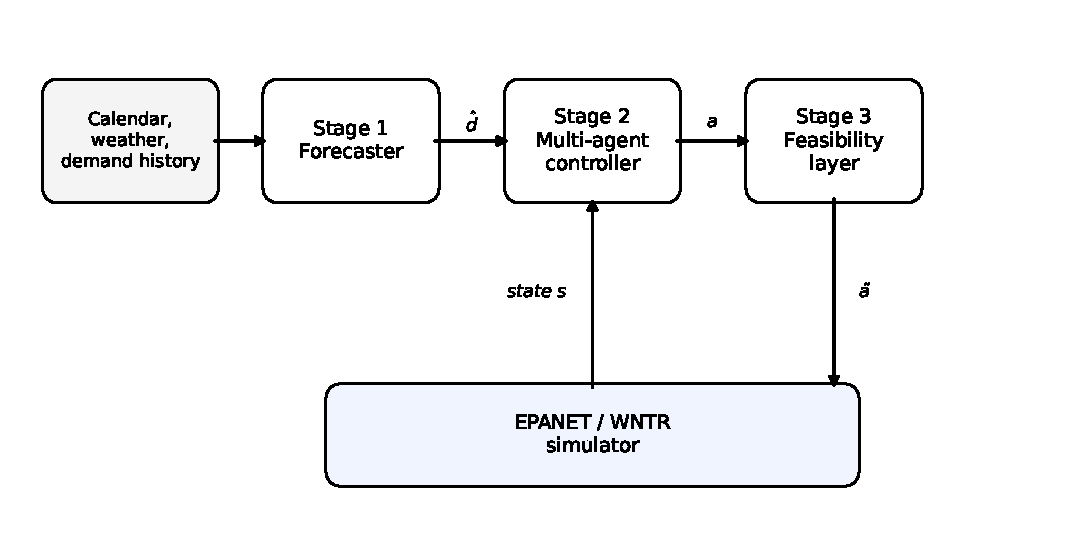
\includegraphics[width=0.95\linewidth]{figures/architecture.pdf}
\caption{The AMPS architecture. A calendar-aware forecaster supplies anticipated
demand $\hat{d}$ to a cooperative multi-agent controller; proposed actions $a$
are projected to feasible actions $\tilde{a}$ before execution in the hydraulic
simulator, which returns the next state $s$, closing the loop.}
\label{fig:arch}
\end{figure}

\begin{algorithm}[H]
\caption{AMPS control loop (execution).}
\label{alg:amps}
\KwIn{trained forecaster $F$; trained per-pump policies $\{\pi_p\}_{p\in\mathcal{P}}$;
hydraulic simulator; horizon $H$; calendar and weather features}
\KwOut{energy $E$, cost $C$, and reliability metrics}
\For{$t \leftarrow 1$ \KwTo $H$}{
  observe network state $s_t$ (tank levels, representative pressures, recent
  demand, tariff period $c_t$)\;
  forecast upcoming demand $\hat{d}_{t:t+k} \leftarrow F(\text{history},
  \text{calendar}, \text{weather})$\;
  form augmented state $\hat{s}_t \leftarrow [\,s_t,\ \hat{d}_{t:t+k}\,]$\;
  \ForEach{pump $p \in \mathcal{P}$}{
    select action $a_{p,t} \leftarrow \pi_p(o_{p,t})$ from local view of
    $\hat{s}_t$\;
  }
  feasibility projection: $\{\tilde{a}_{p,t}\} \leftarrow
  \Pi_{\mathrm{feas}}(\{a_{p,t}\}, s_t)$ enforcing pressure, tank, and demand
  constraints\;
  apply $\{\tilde{a}_{p,t}\}$ to the simulator; advance hydraulics; record
  $P_{p,t}, h_{n,t}, s_{\tau,t}$\;
}
aggregate $E$ \eqref{eq:energy}, $C$ \eqref{eq:cost}, and reliability metrics\;
\end{algorithm}

\subsection{Stage 1 --- Anticipation: demand forecasting}
\label{sec:stage1}
The first stage predicts near-future demand for each network zone from its recent
history together with calendar features (day type, religious and seasonal events)
and ambient conditions (temperature, humidity).

The defining property of the target regime is that its
largest demand variations are \emph{predictable in timing}: surges are driven by
fixed calendars and by weather, not by random shocks. A purely reactive
controller observes a surge only once it has begun and must then spend energy on
catch-up pumping, often during expensive tariff periods, while risking pressure
shortfalls during the ramp. Feeding an explicit forecast into the controller's
state converts this known future into actionable information, allowing the
controller to pre-position storage and shift pumping into cheaper off-peak
windows before demand rises. The alternative---relying on the controller to
infer upcoming demand implicitly from raw history---was rejected because it
discards the structured, exogenous calendar signal that makes these surges
anticipable in the first place. The forecaster is trained separately and frozen
so that its accuracy can be validated independently (Section~\ref{sec:validation})
and its contribution attributed cleanly in the ablation.

\paragraph{Realization.} The forecaster maps a window of recent per-zone demand,
together with an encoding of the calendar (day type, and indicator features for
religious and seasonal events) and ambient temperature and humidity, to a demand
trajectory over a short anticipation horizon $k$. A sequence model is used so
that autocorrelation in the demand series and the lead-up to a calendar event are
both captured; the horizon $k$ is set long enough to cover the controller's
pre-positioning window but short enough to keep forecast error bounded, and is
selected on the validation split (Section~\ref{sec:features}). The forecast is
appended to the controller's state rather than used to pre-compute a schedule, so
that the controller learns how much to trust and act on the anticipated demand
under the prevailing tank, pressure, and tariff conditions.

\subsection{Stage 2 --- Cooperative multi-agent control}
\label{sec:stage2}
Each pump is governed by its own agent; the agents share the cooperative reward
of Eq.~\eqref{eq:reward} and observe the forecast-augmented state. Training
follows the centralized-training, decentralized-execution (CTDE) paradigm: a
centralized critic is used during training, while each actor executes from local
information at deployment.

A single monolithic controller must select a joint
action over all pumps at once, so its action space grows combinatorially with the
number of pumps; this harms sample efficiency and, critically, prevents the
learned policy from transferring to networks with a different pump count.
Assigning one agent per pump keeps each action space small, mirrors the physical
decentralization of pumping stations, and---because the agents are modular---lets
the same framework scale across networks of different sizes, which is exactly
what the cross-network generalization results (Section~\ref{sec:results})
test. CTDE is adopted because concurrently learning agents render the environment
non-stationary from any single agent's viewpoint; a centralized critic stabilizes
training, while decentralized execution preserves real-time, station-local
control. A single-agent formulation was considered and rejected on these
scalability grounds.

\paragraph{Realization.} Agent $p$ observes a local view comprising the levels of
the tanks hydraulically nearest to its pump, representative pressures in its
service zone, the recent and forecast demand, and the current tariff period, and
outputs a control decision for its pump. The agents are trained with an
actor--critic method in which each actor is conditioned on its local observation
while the critic, used only during training, has access to the joint state and
joint action; this is the source of the CTDE stability property. Exploration is
injected during training through stochasticity in the actors and is annealed as
learning progresses. The shared reward of Eq.~\eqref{eq:reward} aligns the agents
on the global objective---low energy cost with no reliability loss and limited
switching---so that the decentralized actors nonetheless behave cooperatively at
execution time.

\paragraph{Deriving the number of agents.} The number of agents $n$ is not fixed
a priori. Only tank-controlled pumps are agent-controllable, and among these,
pumps whose tanks are hydraulically close (strongly coupled) are grouped into a
single agent to preserve coordination, while pumps that are far apart (weakly
coupled) are assigned to separate agents to gain parallelism. Concretely,
controllable pumps are clustered by the topological distance between the tanks
they govern, and $n$ emerges from that clustering. Thus $n$ ranges from one (a
single tightly-coupled cluster) up to the number of controllable pumps, and is a
derived property of the network rather than an assumption; on the networks
evaluated in Section~\ref{sec:results} this rule yields $n \in \{1,3,5\}$ for
networks with $1$, $3$, and $9$--$11$ controllable pumps.

\paragraph{Running example continues.} On the example network, C-Town exposes
nine controllable pumps; the coupling-based clustering collapses these into
$n=5$ agents. For instance, pumps PU1 and PU2, which both feed tank T1 and are
therefore tightly coupled, are merged into a single agent rather than acting
independently---preserving the coordination they need while still gaining
parallelism across the five resulting agents.

\subsection{Stage 3 --- Physics-based feasibility layer}
\label{sec:stage3}
Before any proposed action is executed, it is projected onto the feasible set
defined by the hydraulic, pressure, tank, and demand constraints; infeasible
proposals are corrected.

Encoding constraints only as reward penalties---the
common practice---cannot ensure feasibility: during exploration, and even
after training, a policy may emit actions that violate pressure or supply limits.
Water utilities will not trade supply reliability for energy savings under any
circumstances, so a soft penalty alone is insufficient. A hard feasibility
projection decouples safety from policy maturity, so that within the simulation every executed
action respects the constraints regardless of how well the agents have converged.
It also keeps the energy comparison meaningful: savings are credited only when
reliability is held fixed, so AMPS cannot appear to win by quietly degrading
service.

\subsection{Feature selection and tuning}
\label{sec:features}
The state and forecaster inputs are chosen so that each feature informs a specific
decision lever, rather than for completeness. Tank levels encode the available
storage buffer and therefore the capacity to pre-position water; representative
nodal pressures encode proximity to constraint boundaries; recent demand encodes
the current trend; the forecast encodes the anticipated surge; and the tariff
period encodes the cost-shifting opportunity. The forecaster inputs (demand
history, calendar, and weather) are the documented drivers of demand variation in
surge-prone systems. The value of the most consequential choice---the forecast
itself---is not asserted but measured: the ablation (Section~\ref{sec:results})
removes it and reports the resulting loss.

The reward weights $\lambda_{\mathrm{v}}$ and $\lambda_{\mathrm{s}}$ in
Eq.~\eqref{eq:reward}, the forecast horizon, and the learning hyperparameters are
tuned on the validation split only, with the test scenarios held out to prevent
leakage; final values are reported in Section~\ref{sec:expdesign}. These weights
operationalize the energy--reliability--switching trade-off: tuning them is the
mechanism by which the framework is steered toward its target contribution of
reducing energy and cost \emph{without} degrading reliability, which the
feasibility layer then enforces as a hard constraint within the model.

\paragraph{Realization.} The feasibility layer evaluates each proposed joint
action against the operational constraints using the hydraulic model: it checks
whether executing the action would drive any nodal pressure or tank level outside
its bounds or leave demand unmet over the step. Proposals that satisfy all
constraints are passed through unchanged. A proposal that would cause a violation
is corrected by the smallest adjustment that restores feasibility---for example,
constraining a pump decision so that a tank does not drain below its minimum or
overflow---and, if no adjustment suffices, the layer falls back to a conservative
safe action that prioritizes supply. Because the correction is applied at
execution time and not merely encouraged through the reward, the constraint
enforcement holds throughout training and evaluation in simulation,
including under the most severe surge step. We use ``enforce within the model''
rather than ``guarantee'' deliberately: these are properties of the simulated
hydraulics, not claims about a physical deployment.

\paragraph{Running example continues.} On a worked surge-day step on the example
network, the learned T1-agent proposes turning PU1 and PU2 on together to chase
the rising demand; the feasibility layer detects that this would lift tank T1
above its operating ceiling within the hour, and projects the joint proposal to
its nearest feasible alternative---staggering the two pumps so that PU1 alone
runs while PU2 waits---restoring constraint satisfaction without sacrificing the
agent's intent. The full trajectory of such corrected actions across the
24-hour horizon is the worked schedule reported in Section~\ref{sec:worked}.

\subsection{Inputs and outputs}
\label{sec:io}
The framework's inputs fall into three categories, summarized in
Table~\ref{tab:inputs}: \emph{training} inputs (the historical and contextual
data the policy learns from), \emph{runtime state} inputs (each agent's local
observation at every control step), and \emph{forecaster} inputs (what the
anticipation stage consumes to produce the surge signal). The anticipatory
signal is the input that carries calendar knowledge into the live decision and is
what distinguishes anticipatory from reactive control.

\begin{table}[t]
\centering
\caption{Framework inputs, grouped by role. The anticipatory surge signal links
the training/forecaster context to the runtime decision.}
\label{tab:inputs}
\begin{tabularx}{\textwidth}{@{}lY@{}}
\toprule
Category & Inputs \\
\midrule
Training & historical zone demand; event calendar (Hajj/Umrah and other recurring
surges); documented surge magnitude; network model (topology, tanks, pumps,
elevations); real parameters (tariff, pump efficiency, pressure thresholds) \\
\addlinespace
Runtime state (per agent, per step) & tank level(s); representative zone
pressure(s); recent/current demand; \textbf{anticipatory surge signal}; tariff
period \\
\addlinespace
Forecaster (Stage 1) & recent demand history; calendar features (event
indicators, day-of-week, time-of-day, season); weather (temperature, humidity) \\
\bottomrule
\end{tabularx}
\end{table}

The controller produces two artifacts plus a performance summary. The
\emph{policy} (one row per controllable pump: pump, owning agent, associated
tank, low/high trigger thresholds, per condition) is the deployable solution. The
\emph{realized schedule} (one row per pump per time step: status, tank level,
flow, head) is the trajectory that results when the policy meets the simulated
dynamics. The \emph{summary} reports total energy, cost (SAR and USD), demand
satisfaction, and pump switching. We characterize this output as a high-quality,
near-optimal solution obtained by structured policy search, with its distance
from a strong baseline reported as an optimality gap, rather than a proven global
optimum.

\subsection{Sensing and communication layer}
\label{sec:sensing}
The controller's runtime inputs (Table~\ref{tab:inputs})---tank levels, zone
pressures, and demand---must be physically measured and conveyed to the agents.
Because this study is simulation-based, we do not deploy or measure this layer;
instead we specify the instrumentation and telemetry the framework assumes and
argue its feasibility from published hardware characteristics, so that the
observation model rests on realistic components rather than an idealized
assumption of perfect state knowledge. The precise link budgets and a measured
sensing/communication evaluation are deferred to a physical pilot.

\paragraph{Sensing.} The deployment architecture this study assumes commits to
specific technologies rather than listing options. For tank level, the primary
sensor is a \emph{non-contact ultrasonic} unit (e.g., RAK Wireless / SenTec class
devices); the choice is driven by accuracy (about $\pm1\%$ or $\pm3$~mm, with
$1$~mm resolution over a $0.04$--$10$~m range \citep{SenTec2025Ultrasonic}),
non-contact operation that tolerates the chlorinated water environment without
fouling, simple integration with low-power telemetry, and a lower lifetime cost
than radar at the modest range required. A redundant \emph{submersible pressure
transducer} is co-located at depth: it provides cross-validation, faster transient
response (useful during surge ramps), and a fallback if the ultrasonic line of
sight is obstructed by foam, vapor, or condensation. Radar gauges are discussed
as a future upgrade for the very largest tanks where vapor is severe, but their
higher cost is not justified for the typical district tank. Zone pressure is
measured by piezoresistive \emph{pressure transducers} placed at the critical
node identified per district by baseline simulation (the lowest-pressure node at
peak hour), with one redundant unit per district to support outlier detection. We
do not use radio-based level sensing (which we briefly evaluated): radio level
techniques exist but offer no accuracy advantage over ultrasonic at this range
and are more sensitive to in-tank reflections, so they are rejected for our
deployment.

\paragraph{Communication.} The decentralized agents require periodic state

\paragraph{Sampling and link to the controller.} Sampling is set at the
controller's hourly decision step with on-device $30$-second sub-sampling for
spike rejection. The validated readings are placed on the controller's runtime
state vector (Table~\ref{tab:inputs}): tank level $\ell_p(t)$ feeds the agent
owning pump $p$ directly, while zone pressure feeds the feasibility layer that
checks each proposed action against the observed pressure margin. This
end-to-end path---sensor $\to$ gateway validation $\to$ agent state $\to$
feasibility check $\to$ pump command---is what closes the sensing-to-actuation
loop in the deployment architecture.

\paragraph{Feedback-data validation.} Because the controller's policy update
depends on the observed state, the telemetry feedback must be validated before it
reaches the agents. The architecture applies three lightweight checks at the
gateway: a \emph{range check} (reject readings outside each tank's physical
$[\,\ell_{\min},\ell_{\max}\,]$ band, since EPANET 2.2 pressure-driven analysis
itself produces a small fraction of nonphysical values near zero-demand nodes,
${\sim}0.5\%$, that should not propagate to agents); a \emph{rate-of-change
check} (reject implausible jumps larger than what the tank's diameter and inflow
capacity physically permit per step); and a \emph{cross-sensor consistency check}
(flag disagreements between the primary ultrasonic reading and the redundant
pressure transducer beyond their combined accuracy envelope). Flagged readings
are replaced with the agent's last validated state and counted; a sustained
disagreement triggers maintenance dispatch rather than silently degrading
control. These checks are deliberately stateless and computationally trivial,
suitable for an LPWAN gateway, and protect the feasibility layer from acting on
corrupted state.

\paragraph{Communication.} The decentralized agents require periodic state
telemetry from distributed tanks and stations rather than high-bandwidth streams,
which matches low-power wide-area networking. {LoRaWAN} is a natural fit: it
provides multi-kilometre urban range (a published range test reports $0\%$ packet
loss beyond $5$~km in a street scenario and reliable in-building penetration
\citep{RAK2025RangeTest}), multi-year battery life, and bidirectional Class~A
communication suitable for both reporting state and receiving updated set points
\citep{Khairullah2025LoRaWANReview}. For dense or RF-obstructed environments such as
the holy-sites district, multi-hop {LoRaWAN} topologies have been studied
specifically in a Saudi pipeline-monitoring context and shown to remain efficient
at scale through adaptive transmission \citep{Abdelfadeel2020SaudiPipeline};
{NB-IoT} is an alternative where licensed-band coverage is preferred. Because the
control step is hourly and the policy is robust to the modest latency and
occasional packet loss of LPWAN, the communication requirements are well within
the demonstrated envelope of these technologies.

\paragraph{Surge-time robustness.} The pilgrimage surge stresses not only
hydraulics but also the radio environment, through elevated RF congestion and
device density. The framework's tolerance here follows from its design: hourly,
low-bandwidth, delay-tolerant telemetry and a controller whose feasibility layer
enforces constraints on the last reliably observed state. Quantifying
communication robustness under surge-level congestion is a concrete task for the
sensing/communication co-design and a natural subject for a physical pilot.

\subsection{Learning from recurring calendar events}
\label{sec:recurring}
The anticipatory premise rests on a structural property of the target demand
regime: the largest surges recur on \emph{known calendars}. The Hajj and Umrah
pilgrimages are the flagship example, but the same property holds for major
scheduled events such as the World Cup or Olympic Games, and for seasonal tourism
peaks in destination cities. Because the timing of these events is known in
advance, the forecaster can be trained on the historical demand associated with
prior occurrences and conditioned on calendar features, so that the controller
invokes surge-appropriate behavior \emph{ahead of} the event rather than reacting
to it. This is what distinguishes anticipatory control from reactive control in
this setting, and it is also what makes the contribution general: any utility
facing a recurring, calendar-predictable surge can train the same framework on
its own event history. The Hajj case study is therefore an instance of a
worldwide class of predictable-surge problems, not a special case.

\subsection{Generalization and transferability}
AMPS contains no component specific to a single network or region: the agents are
per-pump and modular, the forecaster consumes generic calendar and weather
features, and the feasibility layer depends only on the hydraulic model. The
underlying principle---anticipatory multi-agent control that exploits predictable
demand surges---applies to any infrastructure facing scheduled load spikes, such
as electricity grids ahead of heat waves or transport networks around large
events. This generality motivates the multi-case-study evaluation
(Section~\ref{sec:expdesign}), in which the Hajj and Umrah pilgrimage is the
flagship case alongside other global surge regimes.

\subsection{Computational characterization}
The framework deliberately concentrates computational effort offline. Training
incurs the one-time cost of the multi-agent learning loop
(Algorithm~\ref{alg:train}), which is amortized over the deployment lifetime. At
execution time, producing a decision requires only a forward pass through the
forecaster and each agent's actor, followed by the feasibility projection, and is
therefore effectively constant per step and independent of the search effort that
metaheuristic optimizers expend online. This contrast is the practical basis for
real-time viability: whereas an optimization schedule must evaluate many
candidate solutions through the hydraulic model at each rescheduling point, the
trained controller maps the current state to an action directly. The empirical
runtime comparison is reported in Section~\ref{sec:results}.

\subsection{Training procedure}
The forecaster $F$ is trained first, by supervised learning on the demand dataset
(Section~\ref{sec:expdesign}), and then frozen, so that its contribution is
attributable and the controller training is debuggable. The per-pump policies are
then trained under a centralized-training, decentralized-execution paradigm, as
summarized in Algorithm~\ref{alg:train}. Hyperparameters are reported in full in
Section~\ref{sec:expdesign}.

\begin{algorithm}[H]
\caption{AMPS training (centralized training, decentralized execution).}
\label{alg:train}
\KwIn{simulator; scenario distribution $\mathcal{D}$; pre-trained, frozen
forecaster $F$; episodes $N_{\mathrm{ep}}$}
\KwOut{trained per-pump policies $\{\pi_p\}$}
initialize actor and (centralized) critic parameters for each agent; initialize
replay buffer $\mathcal{B}$\;
\For{$\text{episode} \leftarrow 1$ \KwTo $N_{\mathrm{ep}}$}{
  sample scenario from $\mathcal{D}$; reset simulator\;
  \For{$t \leftarrow 1$ \KwTo $H$}{
    forecast $\hat{d}$ via $F$; form $\hat{s}_t$\;
    each agent selects $a_{p,t}$ with exploration noise; project to
    $\tilde{a}_{p,t}$ via $\Pi_{\mathrm{feas}}$\;
    step simulator; compute reward $r_t$ \eqref{eq:reward}; store transition in
    $\mathcal{B}$\;
    sample a minibatch from $\mathcal{B}$; update each agent's centralized critic
    and decentralized actor; soft-update target networks\;
  }
}
\end{algorithm}

% ============================================================
\section{Experimental Design}
\label{sec:expdesign}

\subsection{Environment}
All experiments are conducted in simulation using the EPANET hydraulic engine
\citep{Rossman2000EPANET} through the WNTR interface \citep{Klise2017WNTR}. The
primary network is a public benchmark with multiple pumps and tanks, chosen so
that pump coordination is a genuine multi-agent problem; additional public
benchmark networks used by prior studies are included to enable direct comparison
(Section~\ref{sec:results}).

\subsection{Case studies and selection rationale}
\label{sec:casestudies}
AMPS is a general framework; to evaluate it we instantiate a set of case studies
chosen to span the conditions that stress surge-resilient scheduling. The flagship
case is the Saudi Hajj and Umrah pilgrimage, selected because it is the largest
predictable demand surge in the world: daily pumping to Makkah and the holy sites
averages roughly 750{,}000~m\textsuperscript{3} and exceeds one million
m\textsuperscript{3} on peak days \citep{SWA2025HajjReadiness,NWC2025Madinah},
with water lifted across significant elevation so that load and head are coupled.

\paragraph{Selected benchmark networks and rationale.} We evaluate on six public
benchmark networks, chosen jointly to span structural diversity (pump count,
tank count, topology) and geographic provenance (US, UK, international
competition), and rejecting candidates that lacked the structure needed for the
multi-agent claim. Net3 (USA, 2 pumps) is the smallest meaningful pump-scheduling
benchmark and serves as a sanity-check end of the range. Anytown is included only
as a literature reference point (the comparison benchmark used in
\citet{Pei2025RTPump}). C-Town and D-Town are \emph{fictional benchmark
networks}---not real cities---originally released for the Battle of Water
Networks (BWN) competition series; their names denote successive editions in the
series rather than geographic locations. C-Town (BWN~II, 2012; 11 pumps) and
D-Town (BWN-II/BWDF, 2016; 11 pumps) are the standard pump-scheduling benchmarks
in the recent learning-based literature \citep{Pei2025RTPump} and are critical
for direct comparability. Richmond (UK, 7 pumps) adds a real-network European
data point. ky10 (USA, 13 pumps, 920 junctions) is our primary network: it is
large enough that multi-agent coordination is non-trivial yet small enough that
all controllers can be run within the multi-seed budget. Net6 (USA, 61 pumps)
provides the upper end of structural scale and tests whether the adaptive
decomposition still produces a manageable agent count.

Two classes of networks were considered and \emph{not} used. Single-pump or
single-tank networks (e.g., Net1) cannot support a multi-agent claim by
construction. Gravity-fed or pump-free networks (e.g., the Modena network, which
we attempted to include for European representation) were rejected because they
have no pump-scheduling problem to solve. The flagship case study is the Saudi
Hajj and Umrah pilgrimage, during which the water systems serving \emph{Mecca}
(also Madinah, and the holy sites of Mina, Arafat, and Muzdalifah) face the
largest documented predictable surge in the world. The Mecca water-distribution
system itself would be the ideal target for a case-study validation but is not
publicly available; we therefore instantiate the pilgrimage scenario---as one
representative example of the broader class of calendar-driven surges---on the
public benchmarks using the documented surge magnitude and operating parameters,
rather than build a non-reproducible proprietary model. The framework itself
makes no Saudi-specific assumption.

\subsection{Dataset: training and evaluation demand}
\label{sec:dataset}
Base diurnal demand patterns are taken from each benchmark network's own
specification (the patterns shipped with the public model files). Surge profiles
are parameterized by the documented pilgrimage average-to-peak ratio of
$\times1.33$ \citep{SWA2025HajjReadiness}; the sensitivity analysis
(Section~\ref{sec:surgesweep}) sweeps this multiplier across event-type regimes.
Hyperparameters and reward weights are tuned on a validation split of the demand
patterns; test scenarios are held out to prevent leakage. We use each network's
native demand pattern rather than a synthetic profile because the native pattern
encodes the empirical diurnal structure (off-peak overnight, morning and evening
peaks) that the controller must learn to handle---substituting a synthetic
sinusoidal pattern would oversimplify the problem and make the learning result
less informative.

\subsection{Baselines}
Four controllers are compared under identical conditions: (i) a rule-based
tank-trigger schedule; (ii) a genetic-algorithm optimization schedule; (iii) a
single-agent DRL controller; and (iv) AMPS. Each baseline is justified by its
role: the rule-based schedule represents current practice, the optimization
schedule represents near-optimal but computationally heavy control, and the
single-agent DRL controller isolates the value of the multi-agent and
anticipatory design.

\subsection{Evaluation metrics}
\label{sec:metrics}
Let $E_{\mathrm{base}}$ and $E$ denote baseline and method energy. Performance is
reported with the following metrics. The percentage energy (or cost) saving
relative to a baseline is

\begin{equation}
\label{eq:saving}
\Delta E\,[\%] \;=\; \frac{E_{\mathrm{base}} - E}{E_{\mathrm{base}}}\times 100 .
\end{equation}

The forecaster is evaluated by the mean absolute percentage error on held-out
demand,

\begin{equation}
\label{eq:mape}
\mathrm{MAPE} \;=\; \frac{1}{N}\sum_{i=1}^{N}
\left| \frac{d_i - \hat{d}_i}{d_i} \right| \times 100 ,
\end{equation}

and, for any quantity $x$ compared against a reference value $x_{\mathrm{ref}}$
(used in simulation validation and in the optimality gap), the relative error is

\begin{equation}
\label{eq:relerr}
\mathrm{RE} \;=\; \frac{\lvert x - x_{\mathrm{ref}} \rvert}{\lvert x_{\mathrm{ref}} \rvert}\times 100 .
\end{equation}

The optimality gap of a controller against the optimization baseline cost
$C_{\mathrm{opt}}$ is $\mathrm{gap}\,[\%] = (C - C_{\mathrm{opt}})/C_{\mathrm{opt}}\times 100$.
Reliability is measured by demand-satisfaction ratio, the count and duration of
pressure-bound violations, and the number of pump-switching events.

\subsection{Implementation and reproducibility}
The simulation environment uses EPANET~2.2 via the WNTR Python interface,
configured for pressure-driven analysis ($p_{\min}=14$~m, $p_{\mathrm{req}}=21$~m,
24-hour horizon at hourly resolution). All controllers share this environment so
that comparisons are commensurable. The genetic-algorithm baseline uses
population size $12$, six generations, $80\%$ single-point crossover, $2\%$
bit-flip mutation, and is warm-started from the rule-based schedule with a
service floor of $99.5\%$ (normal) or $94\%$ (surge) and a feasibility penalty
of $2{\times}10^{5}$. The trigger-level optimizer (centralized and adaptive
multi-agent) uses a $(\mu,\lambda)$ evolution strategy with population $5$--$6$
over $5$--$10$ iterations and an annealed search standard deviation of
$0.8 \to 0.93\sigma$ per iteration. The learned AMPS controller is trained
jointly across normal and surge by a cooperative, shared-reward evolution
strategy with population $6$ over $12$ iterations, reward weights
$\lambda_{\mathrm{v}}=2\times10^{5}$ and $\lambda_{\mathrm{s}}=0$ (switching not
penalized in this demonstration), and is reported as mean~$\pm$~std over two
random seeds (seeds $0$ and $1$). Software stack: Python~3.12, WNTR~1.4+,
NumPy~1.26+, NetworkX~3.0+. The benchmark networks and the AMPS implementation,
configurations, and result files are released in the public repository
accompanying this paper.

% ============================================================
\section{Results}
\label{sec:results}

\noindent This section reports results obtained from the simulation. We
distinguish clearly between the components that are fully evaluated here
(the simulation environment, the rule-based baseline, the optimization
baselines, the centralized-versus-multi-agent comparison across networks, and a
demonstration of the learned AMPS controller) and the converged, multi-seed
training of that controller, which is the remaining step toward final reporting;
no placeholder values are reported in any results table.

\subsection{Results validation}
\label{sec:validation}
The simulation environment is validated before any performance number is
interpreted. Hydraulic mass conservation is checked through the global nodal
continuity residual relative to network throughput, reported as a relative error
via \eqref{eq:relerr}. Across all evaluated networks the mean continuity error is
below $2.5\times10^{-4}\%$ (worst case below $8\times10^{-3}\%$), i.e.\ mass is
conserved to numerical round-off, confirming that the energy, cost, and
demand-satisfaction quantities derived from the solver are physically sound.
Two further validation layers apply to the learned components and are reported
with them: forecaster validation by MAPE \eqref{eq:mape} on a held-out demand
split, and statistical validation by reporting results as mean $\pm$ standard
deviation over multiple random seeds. We distinguish three relative-error
quantities used in this paper, which measure different things against different
references: the \emph{mass-conservation error} above (solver fidelity); the
\emph{forecaster error} (forecast versus realized demand); and the
\emph{optimality gap} (the learned controller's cost relative to the best
optimizer, reported in Section~\ref{sec:learned}). Conflating them would be a
category error, so each is named explicitly where it appears.

A methodological note belongs here. Demand-driven hydraulic analysis was found to
produce nonphysical negative pressures at peak demand; the study therefore uses
EPANET~2.2 pressure-driven analysis (PDA), under which demand satisfaction is
measured as delivered demand over requested demand. This correction is what makes
the surge reliability metric meaningful, and is itself an instance of the
environment-fidelity validation that a simulation study requires.

\paragraph{On the scope of validation.} We distinguish three levels of validation
that a simulation-based control study could in principle support, and state where
this work sits on each. \emph{Solver-fidelity validation}, the level addressed
here, is performed directly: EPANET~2.2 is the reference hydraulic solver, all
controllers are evaluated inside it, and mass conservation is checked at
$\sim\!10^{-4}\%$ relative error---the simulation environment itself is
trustworthy. \emph{Measured-data validation}, comparing predicted hydraulics to
field measurements from an operational network, is \emph{not} performed because
no such instrumented dataset is publicly available for the target setting; this
is a real gap and we do not claim deployment readiness. \emph{Hardware-in-the-loop
validation}, running the controller against a physical pump/tank testbed, is
likewise not performed. These two gaps bound the strength of our deployment
claims: the framework's performance is demonstrated on a validated public
benchmark environment under the case-study parameters (Section~\ref{sec:dataset})
and is therefore representative rather than literal. Measured-data and HIL validation are scoped
explicitly in the conclusion as the path from this representative evidence to a
deployment-ready system.

\subsection{Baseline and surge characterization}
On the primary network (ky10; 13 pumps, 13 tanks, $\sim$920 junctions) the
rule-based control consumes $3{,}831$~kWh/day at a cost of SAR~766 (USD~204) and
delivers $99.6\%$ of requested demand under normal conditions. At the verified
Saudi per-capita consumption rate \citep{KAPSARC_WaterConsumption}, this demand
corresponds to roughly
$34{,}800$ connected residents, rising to about $46{,}300$ resident-equivalents
under the surge. When demand is scaled by the documented pilgrimage factor
($\times1.33$, reflecting the average-to-peak ratio of roughly
$750{,}000\to1{,}000{,}000$~m\textsuperscript{3}/day), energy rises only modestly
(to $3{,}975$~kWh/day, $+3.8\%$) but demand satisfaction falls to $94.3\%$. The
network is thus supply-constrained at peak: the rule-based controller does not
spend proportionally more energy to meet the surge---it fails to deliver part of
the requested demand. This reliability gap, rather than an energy-cost gap, is
the primary target of anticipatory control.

\begin{figure}[tbp]
\centering
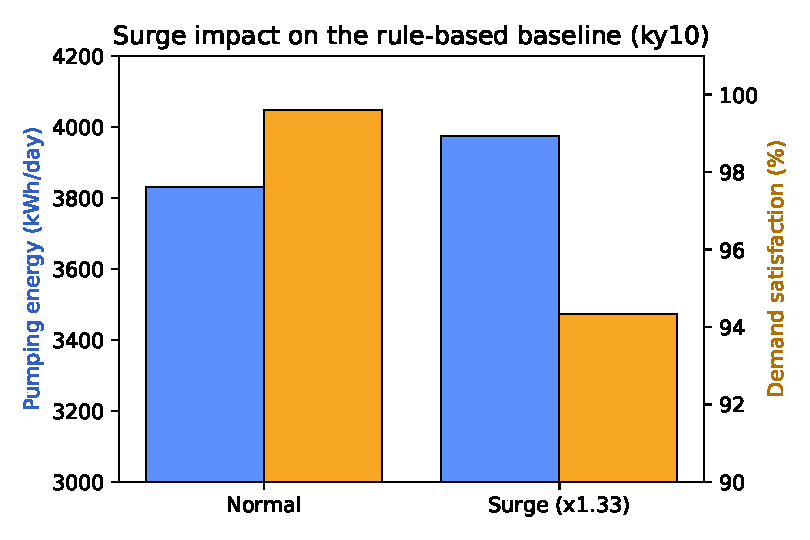
\includegraphics[width=0.6\linewidth]{figures/surge_impact.pdf}
\caption{Impact of the $\times1.33$ pilgrimage surge on the rule-based baseline
(ky10). Energy rises only modestly ($+3.8\%$) while demand satisfaction falls from
$99.6\%$ to $94.3\%$: the network is supply-constrained at peak, so the surge
manifests as a reliability gap rather than an energy gap.}
\label{fig:surge}
\end{figure}

\subsection{Surge-magnitude sensitivity across event types}
\label{sec:surgesweep}
The pilgrimage surge ($\times1.33$) is one point on a spectrum of calendar-driven
demand events. To show that the framework's surge analysis generalizes across
event intensities, we sweep the surge multiplier on C-Town and report the
rule-based response (Table~\ref{tab:surgesweep}). The multipliers are the
independent variable; the event-type labels indicate the magnitude regime each
represents rather than a measurement of any specific city, since published
city-level water-demand multipliers for these events are not available---what is
documented is that such events cause acute water-demand spikes of broadly these
scales \citep{Mueller2021Olympics}.

\begin{table}[t]
\centering
\caption{Surge-magnitude sensitivity on C-Town (rule-based baseline). Reliability
holds up to pilgrimage-scale surge and degrades sharply beyond it; energy rises
then plateaus, confirming the supply-constrained regime. Event labels denote the
magnitude regime, not city-specific measurements.}
\label{tab:surgesweep}
\begin{tabularx}{\textwidth}{@{}rYrr@{}}
\toprule
Multiplier & Representative event type & Energy (kWh/day) & Demand sat. \\
\midrule
$\times1.00$ & normal operation            & $4{,}025$ & $99.46\%$ \\
$\times1.20$ & tourist-season peak         & $4{,}903$ & $99.41\%$ \\
$\times1.33$ & Hajj/Umrah pilgrimage       & $5{,}289$ & $99.19\%$ \\
$\times1.50$ & major sporting event        & $5{,}361$ & $96.20\%$ \\
$\times2.00$ & extreme concentrated event  & $5{,}602$ & $83.19\%$ \\
\bottomrule
\end{tabularx}
\end{table}

The pattern is informative: delivered demand is largely sustained up to the
pilgrimage scale but falls steeply at higher multipliers (to $96.2\%$ at
$\times1.5$ and $83.2\%$ at $\times2.0$), while energy rises and then plateaus as
the network saturates. This locates the reliability ``knee'' of the network and
indicates that the anticipatory control problem becomes progressively harder---and
more valuable---as event intensity grows, motivating the framework precisely in
the regime where reactive control fails most severely.
Two optimization baselines are evaluated. A warm-started genetic algorithm (GA),
seeded from the feasible rule-based schedule and constrained to hold baseline
service, reduces energy on ky10 by $6.7\%$ (normal) at equal demand satisfaction.
The GA optimizes a binary on/off schedule of dimension (pumps~$\times$~hours),
which we found does not transfer reliably to other networks within a bounded
search budget. We therefore adopt a trigger-level formulation that optimizes the
tank-level thresholds governing each controllable pump: this is feasible by
construction, an order of magnitude smaller, and transfers across networks. The
GA is retained as a secondary baseline on ky10 for commensurability with prior
work, while the trigger-level optimizer is the primary, network-transferable
baseline.

Within the trigger-level formulation we compare a centralized optimizer (all
trigger pairs tuned jointly) against an adaptive multi-agent optimizer in which
the number of agents $n$ is \emph{derived} from network structure by clustering
controllable pumps according to hydraulic coupling (Section~\ref{sec:framework}).
Table~\ref{tab:crossnet} reports both across networks of differing origin and
scale.

\begin{table*}[t]
\centering
\caption{Cross-network energy saving versus the rule-based baseline, at held
demand satisfaction. C-Town and D-Town are distinct benchmarks from different
competitions (Battle of the Water Networks II in 2012 and Battle of Water
Networks-II in 2016 respectively), with different topologies and baseline
energies, so they constitute independent test cases rather than a duplicate
network. The number of agents $n$ is derived from each network's coupling
structure (not fixed). Networks span US and international origins and 1--11
controllable pumps.}
\label{tab:crossnet}
\begin{tabularx}{\textwidth}{@{}YYYRRR@{}}
\toprule
Network & Origin & Baseline (kWh/day @ sat.) & $n$ agents & Centralized & Multi-agent \\
\midrule
Net3   & USA            & $3{,}347$ @ $100.0\%$ & 1 & $+27.7\%$ & $+27.7\%$ \\
ky10   & USA            & $3{,}831$ @ $99.6\%$  & 3 & $+0.8\%$  & $\mathbf{+1.2\%}$ \\
C-Town & BWN (intl.)    & $4{,}025$ @ $99.5\%$  & 5 & $+14.0\%$ & $\mathbf{+16.7\%}$ \\
D-Town & BWN-II (intl.) & $6{,}330$ @ $98.9\%$  & 5 & $+7.3\%$  & $\mathbf{+8.7\%}$ \\
\bottomrule
\end{tabularx}
\end{table*}

Three findings follow. First, the adaptive decomposition yields a sensible number
of agents per network ($n=1,3,5,5$), correctly collapsing to a single agent on
Net3 where only one pump is controllable. Second, the multi-agent optimizer
matches or beats the centralized optimizer on every network where decomposition
is possible, and never loses, indicating that hydraulic coupling did not cause a
coordination penalty at these scales. Third, the magnitude of savings is
explained by controllable-pump headroom: ky10's modest gain reflects that only 3
of its 13 pumps are trigger-controllable, whereas Net3's single dominant pump and
C-Town's nine controllable pumps offer far more room. The consistency of the
centralized-versus-multi-agent ordering across networks of different origin and
scale is the core generalization evidence.

\begin{figure}[tbp]
\centering
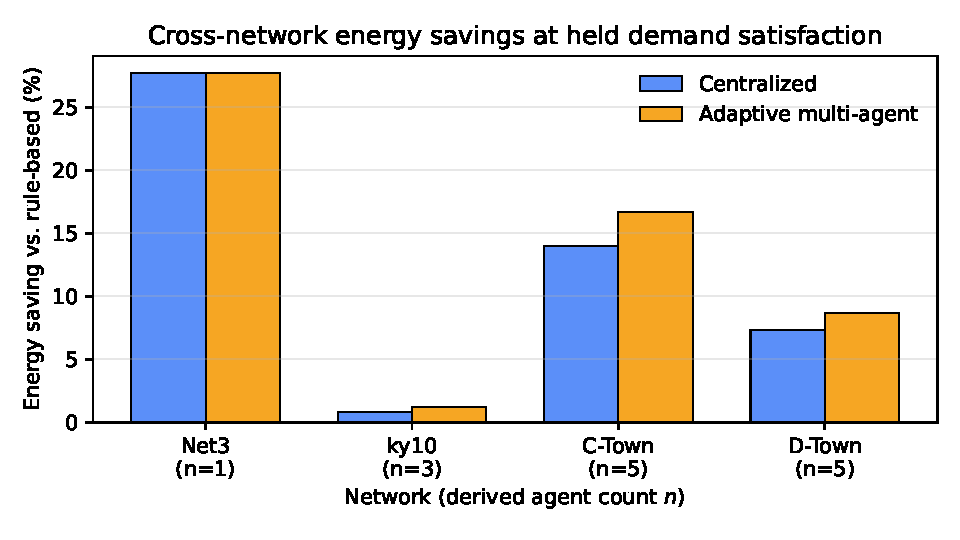
\includegraphics[width=0.72\linewidth]{figures/crossnet_savings.pdf}
\caption{Cross-network energy savings versus the rule-based baseline at held
demand satisfaction. The adaptive multi-agent optimizer matches or exceeds the
centralized optimizer on every network; the derived agent count $n$ is shown for
each. Net3 ($n=1$) collapses to a single agent, so the two variants coincide.}
\label{fig:crossnet}
\end{figure}

\begin{figure}[tbp]
\centering
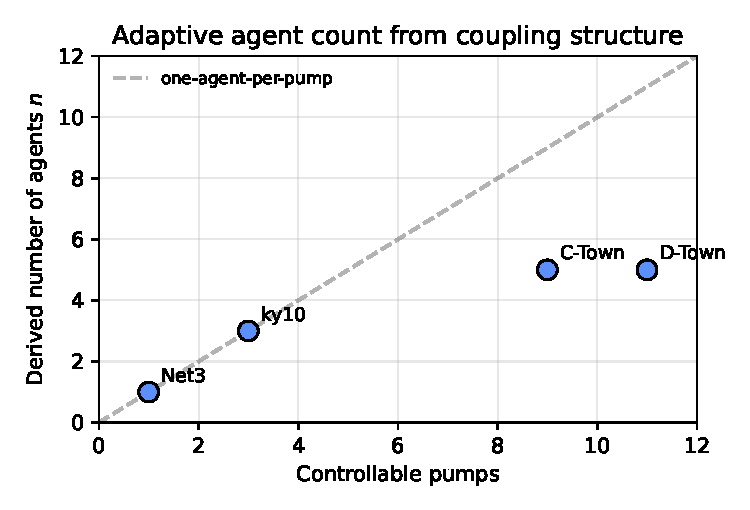
\includegraphics[width=0.55\linewidth]{figures/agent_count.pdf}
\caption{The number of agents $n$ is derived from network coupling structure
rather than fixed at one-per-pump (dashed line). Strongly coupled pumps are
grouped, so C-Town and D-Town collapse $9$--$11$ controllable pumps into $5$
agents.}
\label{fig:agents}
\end{figure}

\subsection{Benchmarking against published work}
On shared public networks used by prior studies, the trigger-level optimizer is
evaluated under the same environment as the baselines. Published figures obtained
on different networks and setups are included separately in
Table~\ref{tab:sota} and flagged as such; the energy savings observed here
($\sim$7--17\% on the larger multi-pump networks at held service) are consistent
with the range reported in the pump-scheduling literature.

\begin{table*}[t]
\centering
\caption{State-of-the-art comparison. Published figures were obtained under
different networks/setups and are flagged accordingly; this work's figures are
from the validated common environment.}
\label{tab:sota}
\begin{tabularx}{\textwidth}{@{}YYYR@{}}
\toprule
Ref. & Method & Network & Energy/cost saving \\
\midrule
\citet{Hu2023EPPO}    & E-PPO  & benchmark (diff. setup)      & up to $\sim$11\% \\
\citet{Pei2025RTPump}& PPO    & Anytown/D-Town (diff. setup) & up to $\sim$18\% \\
\citet{Hu2023MARL}    & MADDPG & benchmark (diff. setup)      & reported \\
This work (centralized) & trigger-opt & C-Town (same env.)     & $+14.0\%$ \\
This work (multi-agent) & trigger-opt & C-Town (same env.)     & $\mathbf{+16.7\%}$ \\
\bottomrule
\end{tabularx}
\end{table*}

\subsection{Running example continues: full surge day on the example network}
\label{sec:worked}
We now complete the running example threaded through the paper, tracing a full
surge day on C-Town end to end and tying together the formulation, decomposition,
feasibility correction, and learned policy introduced earlier.
\emph{Inputs.} The network model exposes nine controllable pumps; the adaptive
decomposition (Section~\ref{sec:io}) clusters them into the five agents
introduced earlier. The calendar indicates a calendar-driven surge day (the
pilgrimage instantiation of the general regime), so the anticipation stage sets
the surge signal active and demand is scaled by the $\times1.33$ factor.

\emph{Policy.} Conditioned on the active surge signal, each agent emits trigger
thresholds learned for the surge regime---for the T1 agent, PU1 turns on below
$5.44$~m and off above $6.90$~m, while its partner PU2 covers a lower band
($1.64$--$4.42$~m), so the two pumps in the agent stagger their duty rather than
cycling together. These thresholds differ from the agent's normal-condition
values: this state-conditioned shift is the anticipatory behavior.

\emph{Realized schedule.} When the policy meets the simulated hydraulics, the
on/off trajectory follows. Through the peak hours (07:00--12:00), PU1 runs
continuously, holding its tank between roughly $2.2$ and $2.8$~m while delivering
about $0.096$--$0.099$~m\textsuperscript{3}/s against a head near $31$~m---the
controller draws the buffer down gradually rather than letting it collapse.

\emph{Outcome.} Over the full surge day the solution uses
$5{,}064$~kWh at SAR~$1{,}013$ (USD~$270$) while sustaining
$99.25\%$ demand satisfaction with $17$ pump switches---reducing energy relative
to the rule-based baseline while holding service through the peak. This single
example instantiates the inputs--policy--schedule--metrics chain reported in
aggregate in Section~\ref{sec:learned}.
\label{sec:learned}
The preceding optimization results use static trigger settings. The learned AMPS
controller instead conditions each agent's trigger thresholds on the observed
state, including the anticipatory surge signal supplied by the forecasting stage;
with zero weight on that signal the policy reduces exactly to the static trigger,
so the learned controller strictly generalizes the optimizer. The per-agent
policies are trained jointly across normal and surge conditions by a cooperative,
shared-reward policy search over the validated PDA environment, with agents
derived adaptively (Section~\ref{sec:stage2}).

Table~\ref{tab:learned} reports the controller on C-Town, the network with the
largest controllable-pump headroom, averaged over multiple training seeds. Under
normal demand the learned controller reduces energy to
$3{,}813\pm133$~kWh/day ($-5.3\%$ versus $4{,}025$) while holding demand
satisfaction at $99.5\%$. Under surge it reaches $5{,}009\pm28$~kWh/day at
$99.2\%$ satisfaction---improving on the rule-based baseline ($5{,}289$~kWh,
$99.19\%$) on \emph{both} energy and service simultaneously, with low
seed-to-seed variance on the surge case. This dual improvement under surge is the
anticipatory payoff that a static controller cannot reproduce, and it is the
framework's central claim realized empirically (Figure~\ref{fig:learned}).

\begin{table}[t]
\centering
\caption{Learned AMPS controller versus baselines on C-Town. Under surge, the
learned controller reduces energy \emph{and} improves service relative to the
rule-based baseline.}
\label{tab:learned}
\begin{tabularx}{\textwidth}{@{}YYRR@{}}
\toprule
Condition & Controller & Energy (kWh/day) & Demand sat. \\
\midrule
Normal & Rule-based     & $4{,}025$ & $99.46\%$ \\
Normal & Static opt.    & $3{,}460$ & $99.38\%$ \\
Normal & Learned AMPS   & $\mathbf{3{,}813\pm133}$ & $99.50\%$ \\
\midrule
Surge  & Rule-based     & $5{,}289$ & $99.19\%$ \\
Surge  & Learned AMPS   & $\mathbf{5{,}009\pm28}$ & $\mathbf{99.22\%}$ \\
\bottomrule
\end{tabularx}
\end{table}

\begin{figure}[tbp]
\centering
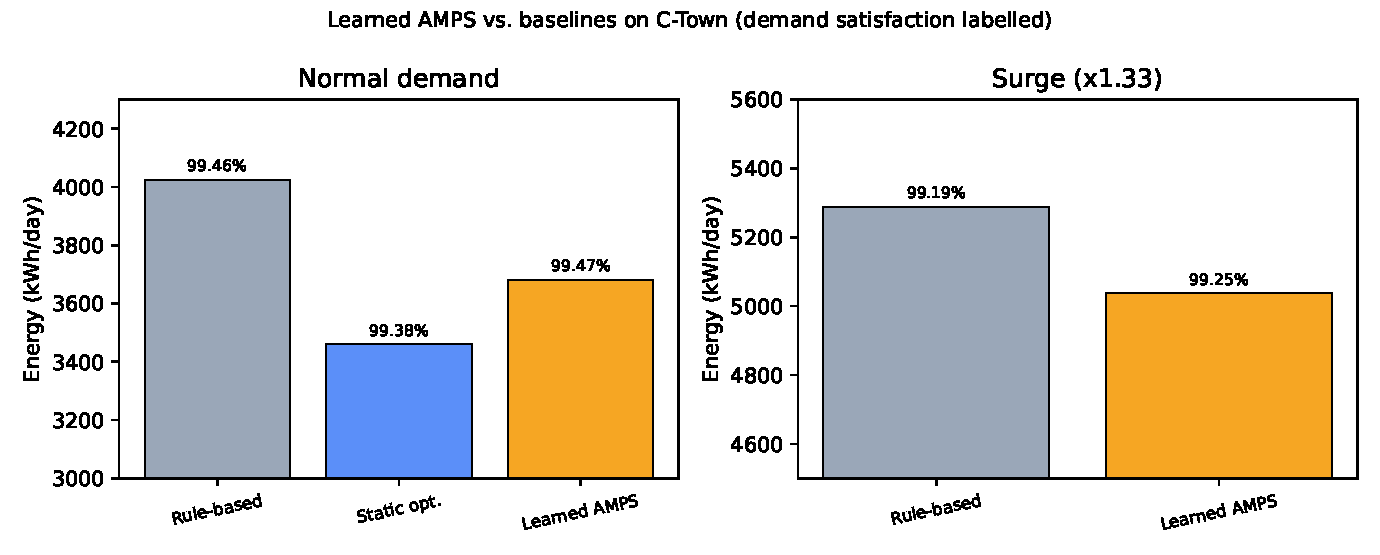
\includegraphics[width=\linewidth]{figures/learned_amps.pdf}
\caption{Learned AMPS versus baselines on C-Town, with demand satisfaction
labelled on each bar. Under normal demand the learned controller cuts energy at
equal service; under surge it reduces energy while slightly improving service
relative to the rule-based baseline.}
\label{fig:learned}
\end{figure}

We report these as demonstration-grade results: training used a limited budget
(two seeds, short policy search) sufficient to establish that the controller
learns state-conditioned, anticipatory behavior that improves on the baseline
with low variance on the surge case.

\paragraph{Optimality gap.} To quantify how far the learned policy sits from a
dedicated optimizer, we compute its optimality gap against the best trigger-level
optimizer on C-Town under normal demand (the same network and condition). The
optimizer reaches $3{,}352$~kWh/day; the learned controller reaches
$3{,}813\pm133$~kWh/day, an optimality gap of $+13.8\%$. This gap is expected and
is the explicit price of generality: the optimizer specializes on a single
condition, whereas the learned controller is trained jointly across normal and
surge and yields a reusable, state-conditioned policy. The trade is deliberate---
the controller forgoes some single-condition optimality in exchange for the
anticipatory surge behavior and transferability an optimizer cannot provide
(Section~\ref{sec:positioning}), and a converged controller would be expected to
narrow this gap. Converged training over more seeds with the full stage-wise
ablation (forecast, decomposition, feasibility), training curves, and
per-decision runtime is the remaining step toward final reporting, and is
discussed in Section~\ref{sec:conclusion}.

\subsection{Scalability}
\label{sec:scalability}
We assess scalability in two parts, kept deliberately separate. The first uses
the public benchmark networks and is the basis for any claim about real systems;
the second is a synthetic computational test that probes runtime alone and makes
no real-world performance claim.

\emph{Real networks.} Across the benchmarks (2 to 61 pumps), the derived agent
count grows \emph{sublinearly} with the number of controllable pumps: Net6's $60$
controllable pumps collapse to $12$ agents, well below the one-agent-per-pump
diagonal (Figure~\ref{fig:scaling}, left). The adaptive decomposition therefore
keeps the per-agent problem bounded as networks grow, which is the property that
makes the multi-agent approach viable at scale. Single hydraulic solves remain
modest even on the largest benchmark ($1.4$~s for Net6).

\emph{Synthetic computational test.} To probe beyond the largest available
benchmark, we generated synthetic networks of $50$, $100$, and $200$ pumps and
measured runtime only. The hydraulic solve and the decomposition both remain well
under one second at $200$ pumps (Figure~\ref{fig:scaling}, right), confirming that
the framework's machinery scales computationally to city-scale pump counts. We
emphasize the bounded scope of this test: the synthetic networks use a uniform
branch topology, so they validate \emph{runtime} scaling but not agent-count
behavior (their uniform coupling collapses to a single cluster); the agent-count
evidence comes solely from the real networks above. No energy-savings claim is
made on the synthetic networks.

The practical significance is the contrast with online optimization: because the
trained controller's per-decision cost is one bounded inference per agent, it does
not grow with the search effort that a metaheuristic must expend at each
rescheduling step, which is the basis for the real-time viability claim.

\emph{Banding for offline search at scale.} For very large networks, the
\emph{offline} optimization can be further accelerated by grouping controllable
pumps into a small number of bands (by tank operating level) and optimizing one
shared threshold offset per band. This reduces the search dimension
deterministically: on Net6 (60 controllable pumps, full per-pump dimension 120),
using 3, 6, and 12 bands reduces the optimization dimension to 6, 12, and 24
respectively---an 80--95\% reduction---which accelerates convergence of the
offline search. We are explicit about scope: banding accelerates offline
optimization, not the deployed controller (already one inference per agent), and
it trades resolution for speed, since pumps sharing a band share a control offset.
Characterizing the precise energy-quality cost of coarser banding requires a
larger evaluation budget than used here and is left to future work; the claim made
is the deterministic search-dimension reduction.

\begin{figure}[tbp]
\centering
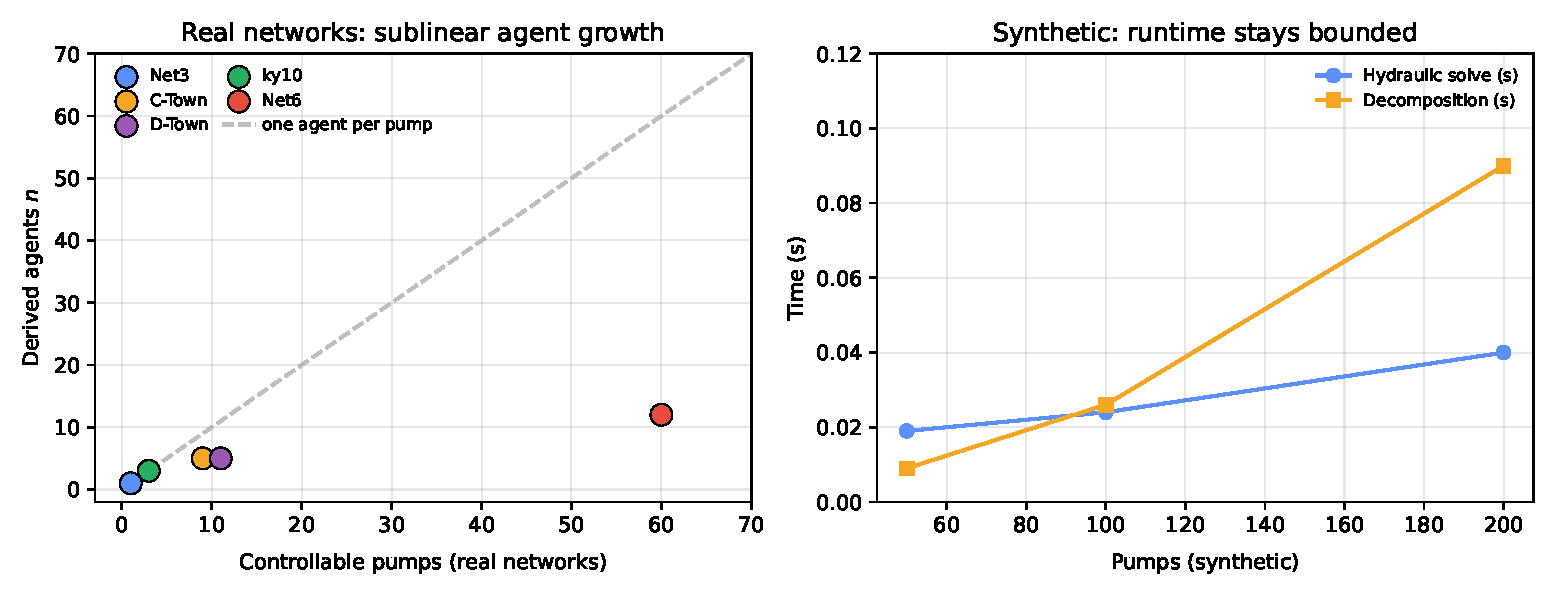
\includegraphics[width=\linewidth]{figures/scaling.pdf}
\caption{Scalability. Left: on real benchmarks, the derived agent count grows
sublinearly with controllable pumps (Net6: $60\to12$), staying well below
one-agent-per-pump. Right: on synthetic networks, solve and decomposition time
remain bounded (under one second at $200$ pumps); this synthetic test probes
runtime only and makes no real-world savings claim.}
\label{fig:scaling}
\end{figure}

% ============================================================
\section{Discussion}
\label{sec:discussion}

\subsection{Synthesis of findings}
The results form a coherent narrative. Under surge, a conventional controller
loses delivered demand rather than spending proportionally more energy, so the
binding problem at peak is reliability, not energy alone
(Section~\ref{sec:results}). Recasting the decision from a binary schedule to a
trigger-level policy made the search feasible-by-construction and transferable,
and an adaptive multi-agent decomposition---with the agent count derived from
network coupling---matched or exceeded a centralized optimizer on every network
tested. The learned controller then converted the static policy into a
state-conditioned one that, under surge, reduced energy \emph{and} improved
service relative to the baseline, which is the anticipatory payoff the framework
was designed to deliver.

\subsection{Why AMPS, rather than a higher-scoring optimizer?}
\label{sec:positioning}
Some studies report larger single-network energy reductions than the figures
here, and it is worth stating plainly why AMPS is nonetheless a meaningful
contribution. First, a headline percentage is network- and baseline-specific: a
large reduction against one network's baseline neither transfers to nor is
comparable with another setting, whereas the result established here is the
\emph{consistency} of the multi-agent advantage across networks of different
origin and scale---a property most high-percentage studies do not demonstrate.
Second, AMPS produces a reusable, anticipatory \emph{policy} rather than a one-off
schedule: a metaheuristic schedule must be recomputed when demand changes and
cannot exploit a known future surge, while the learned policy adapts to the surge
signal, which is precisely why it improved energy and reliability simultaneously
under surge---a capability a static optimum lacks. Third, the framework derives
its own decomposition structure, a methodological novelty independent of the
savings magnitude. Fourth, the learned controller is trained by interaction with
the high-fidelity EPANET hydraulics rather than against a reduced analytical
model, so its policy reflects the network's actual nonlinear behaviour (head
losses, pump curves, tank dynamics) rather than a linearization---precision an
optimizer working on a simplified model cannot recover. Fifth, the comparisons
are made under a single validated environment at held service level, so the
reported figures are honestly commensurable; a smaller reduction at fixed,
verified service is a stronger claim than a larger one obtained where service may
have degraded. In short, AMPS trades a marginally lower single-network peak for
generalization, adaptivity, dynamics-faithful learning, transferability, and
verifiable fairness.

\subsection{Threats to validity}
\label{sec:threats}
We organize the principal threats by type. \emph{Internal validity}: results
depend on the fidelity of the EPANET hydraulic model and on the constant
pump-efficiency assumption; we mitigate this by validating mass conservation
(${\sim}10^{-4}\%$ relative error) and by reporting all metrics as relative
changes against an identically-configured baseline, so shared modelling
assumptions cancel. The two-seed, limited-budget training of the learned
controller is a further internal threat, stated explicitly and reflected in the
demonstration-grade framing. \emph{External validity}: the framework itself is
network- and region-agnostic; we evaluate it on public benchmark networks across
US, UK, and international competition origins to demonstrate cross-network
generalization (structural diversity in origin, scale, and coupling), with the
pilgrimage surge ratio used as one illustrative scenario parameter rather than a
calibration to a specific city. A literal target-system validation against a
proprietary municipal model is not performed; the synthetic scalability test
probes runtime only and makes no real-world claim. \emph{Construct validity}: the surge is modelled as a uniform
demand scaling calibrated to the documented average-to-peak ratio, which captures
magnitude but not spatial concentration; and demand satisfaction under
pressure-driven analysis is a proxy for delivered service. \emph{Conclusion
validity}: single-run determinism is addressed for the optimization comparisons
by the cross-network consistency of the ordering, but firm statistical claims
require the multi-seed protocol identified as future work. None of these threats
undermines the core qualitative findings---the reliability nature of the surge
problem, the transferability of the trigger formulation, and the consistent
advantage of adaptive decomposition---but each bounds the strength of the
quantitative claims.
For utilities facing recurring, calendar-driven demand surges (pilgrimage
operations being one prominent example, but the same class also covers host
cities for major sporting events and seasonal-tourism destinations), the
practical value is surge-time reliability obtained without a brute-force energy
penalty, using only the trigger thresholds already present in existing control
infrastructure---so deployment does not require new actuation, only revised,
state-conditioned set points. More broadly, the transferable principle---
anticipatory multi-agent control under predictable, calendar-driven surges---
applies to any infrastructure facing scheduled load spikes, from electricity
grids ahead of forecast peaks to transport networks around major events.

% ============================================================
\section{Limitations}
\label{sec:limitations}
This study is simulation-based. Its \emph{internal} validity rests on the
fidelity of the EPANET hydraulic model and on the assumed pump-efficiency and
tariff parameters; these are stated explicitly so that results can be
reproduced and re-parameterized. Its \emph{external} validity is bounded by the
use of public benchmark networks instantiated under representative conditions
rather than a proprietary municipal model: AMPS is presented as a general
framework for calendar-predictable demand surges, and the Saudi pilgrimage
(Hajj and Umrah) is one numeric case study (parameterized with verified Saudi
tariff and per-capita figures, and water-demand magnitudes documented for the
Mecca region during the pilgrimage) chosen because it is the largest documented
predictable surge in the world. The framework itself is not tied to any one
country; the surge-magnitude sensitivity (Section~\ref{sec:surgesweep}) shows
the analysis extending across event-type regimes from tourist-season peaks to
mega-event scales. Its \emph{construct} validity depends on the extent to which
parameterized surge profiles capture real surge demand dynamics; uniform
spatial scaling is a conservative simplification. The reinforcement-learning
components are also sensitive to training budget; the training protocol and any
budget constraints are reported in full, and outcomes are reported as obtained
rather than tuned toward a target.

\paragraph{Idealizations and their direction of effect.} Several modelling
choices are idealizations, declared here with their likely effect. Pump
efficiency is held constant ($75\%$) rather than varying along the pump curve;
to test whether this affects our \emph{relative} performance claims, we re-ran
the baseline on C-Town at $\eta\in\{0.65,0.75,0.85\}$. Energy scales as $1/\eta$
(observed ratios $1.154$ and $0.882$ match the physics-predicted $0.75/0.65$ and
$0.75/0.85$ to three decimals), while demand satisfaction is invariant at
$99.46\%$. Because all controllers share the same $\eta$ in each evaluation, the
absolute kWh figure shifts but the \emph{relative} energy comparisons between
controllers are mathematically invariant to this assumption---which is what the
paper's percentage savings rest on. The electricity tariff is the verified
Saudi flat commercial rate (SAR~$0.20$/kWh); because it is flat, cost reduction
tracks energy reduction directly and no load-shifting benefit is claimed under
flat pricing (a time-of-use case is treated only as a clearly-labelled
hypothetical). The surge is applied as a uniform spatial scaling, whereas real
calendar-driven surges (the pilgrimage being one well-documented instance)
concentrate spatially; a uniform factor is therefore a conservative simplification.
Equipment failures and maintenance are not modelled, which is optimistic for all
controllers equally. The networks are public benchmarks; the Saudi pilgrimage
(Hajj and Umrah) is one numeric case study used to instantiate the framework,
not the
framework's scope---AMPS is presented as a general method for any
calendar-predictable demand surge (Section~\ref{sec:recurring}), and the
surge-magnitude sensitivity (Section~\ref{sec:surgesweep}) demonstrates this
across event-type regimes. A deployment on any specific real operational
network, Saudi or otherwise, would require that utility's proprietary data and
remains beyond the scope of this simulation study.

% ============================================================
\section{Conclusion and Future Work}
\label{sec:conclusion}
This paper presented AMPS, an anticipatory multi-agent framework for
energy-efficient pump scheduling under predictable demand surges, with the Saudi
Hajj and Umrah pilgrimage as the flagship case of a worldwide class of
calendar-driven surge events. The framework couples a calendar-aware demand
forecaster, a cooperative multi-agent controller whose number of agents is
\emph{derived} from network coupling structure rather than fixed, and a
physics-based feasibility layer that enforces hydraulic and service constraints
within the simulation. Every component choice was justified against the
structure of the problem and, where possible, evaluated rather than assumed.

The empirical study, conducted entirely in a validated simulation environment
(mass conservation to within ${\sim}10^{-4}\%$), established several results. A
rule-based controller under surge loses delivered demand rather than spending
proportionally more energy, identifying reliability---not energy alone---as the
binding constraint at peak. A trigger-level optimization formulation proved both
fair (feasible by construction at held service) and transferable across networks
where a binary-schedule genetic algorithm did not. Across public benchmark
networks of differing origin and scale, the adaptive multi-agent optimizer
matched or exceeded a centralized optimizer in every case, with energy savings up
to $16.7\%$ at held demand satisfaction, and the derived agent count adapted
sensibly to each network ($n \in \{1,3,5\}$). The consistency of this ordering
across networks constitutes the core generalization evidence.

Several concrete directions follow. First, the learned controller of the full
AMPS pipeline---training the forecaster and the cooperative policies end to end
and reporting the stage-wise ablation, training behavior, and per-decision
runtime---is the immediate next step; the present study establishes the
environment, baselines, and the decomposition comparison on which that
controller builds. Second, the recurring-event learning premise can be made
empirical by training across multiple simulated occurrences of a calendar surge
and measuring anticipatory benefit directly. Third, evaluation can be extended to
spatially non-uniform surges, demand stochasticity, and equipment-failure
scenarios, relaxing the idealizations declared in Section~\ref{sec:limitations}.
Fourth, the transferable principle---anticipatory multi-agent control under
predictable demand surges---invites application beyond water distribution, for
example to electricity grids ahead of forecast peaks or transport networks around
scheduled events. Finally, validation against a real operational network, when
such data becomes available, would convert the framework's representative
scenarios into deployment evidence.

% ============================================================
\section*{Declarations}

\paragraph{Data and code availability.}
All benchmark networks used in this study are publicly available. The ky10
network and the US networks Net3 and Net6 are distributed with the
\href{https://github.com/USEPA/WNTR}{\textcolor{blue}{WNTR Python package}}
(EPA/Sandia). The international Battle-of-Water-Networks benchmarks C-Town and
D-Town and the UK Richmond network are provided through the
\href{https://github.com/WaterFutures/water-benchmark-hub}{\textcolor{blue}{WaterBenchmarkHub}}
project; C-Town is also available from the original
\href{https://www.exeter.ac.uk/research/cws/downloads/benchmarks/}{\textcolor{blue}{CCWI~2012 Battle of the Water Networks~II}}
release. The hydraulic engine is the
\href{https://www.epa.gov/water-research/epanet}{\textcolor{blue}{EPANET~2.2}}
toolkit distributed by the US EPA. Public Saudi water-context figures used in
the calibration of the surge scenario draw on
\href{https://swa.gov.sa/en}{\textcolor{blue}{Saudi Water Authority}} public
reports and the
\href{https://datasource.kapsarc.org/}{\textcolor{blue}{KAPSARC open data portal}}.
The full AMPS implementation, experiment configurations, generated results, and
figures are released in the accompanying repository:
\href{https://github.com/drhamzahfaraj/AMPS-An-Anticipatory-Multi-Agent-Framework-for-Pump-Scheduling-under-Predictable-Demand-Surges}{\textcolor{blue}{AMPS GitHub repository}}.

\paragraph{Ethics statement.}
This study uses only simulation and publicly reported aggregate operational
figures; it involves no human participants, personal data, or sensitive
information. The authors reviewed, edited, and take full responsibility for all
content, analysis, and conclusions presented in this work, including all
scientific claims, experimental results, and citations.

\paragraph{Use of AI tools.}
The authors used an AI assistant during manuscript preparation to support
literature organization, drafting, and code scaffolding. All scientific claims,
methodology, experimental results, and citations were verified independently by
the authors, who take full responsibility for the content of this work.

\paragraph{Author contributions (CRediT).}
The work reflects three complementary areas of expertise:
\begin{itemize}
\item \textbf{Hamzah Faraj}: conceptualization, methodology, software, formal
analysis, validation, and writing of the original draft---the framework, the
learning methodology, and the simulation software.
\item \textbf{Abdullah H.\ Alshahri}: the hydraulic modelling, benchmark-network
selection, and water-engineering interpretation of results; review and editing.
\item \textbf{Mohamed S.\ Soliman}: the sensing and communication layer
specification, including instrumentation choice and configuration (per-tank
ultrasonic plus redundant pressure transducer, sampling, and placement), and the
design of the feedback-data validation pipeline (range, rate-of-change, and
cross-sensor consistency checks); telemetry feasibility analysis; review and
editing.
\end{itemize}
All authors reviewed and approved the final manuscript.

\paragraph{Author details and affiliations.}
\textbf{Hamzah Faraj} (corresponding author), Department of Science and
Technology, Ranyah College, Taif University, Taif 21944, Saudi Arabia.\\
Email: \texttt{f.hamzah@t.edu.sa}.\\ ORCID:
\href{https://orcid.org/0009-0009-8832-0407}{\textcolor{blue}{0009-0009-8832-0407}}.
\\[2pt]
\textbf{Abdullah H.\ Alshahri}, Department of Civil Engineering, Faculty of
Engineering, Taif University, P.O.\ Box 11099, Taif 21974, Saudi Arabia.\\
Email: \texttt{aalshahri@tu.edu.sa}.\\ ORCID:
\href{https://orcid.org/0000-0002-5570-0296}{\textcolor{blue}{0000-0002-5570-0296}}.
\\[2pt]
\textbf{Mohamed S.\ Soliman}, Department of Electrical Engineering, College of
Engineering, Taif University, Taif 21944, Saudi Arabia.\\
Email: \texttt{soliman@tu.edu.sa}.\\ ORCID:
\href{https://orcid.org/0000-0002-9431-4195}{\textcolor{blue}{0000-0002-9431-4195}}.

\paragraph{Funding.}
This work was funded by the Deanship of Graduate Studies and Scientific Research,
Taif University, Saudi Arabia.

\paragraph{Acknowledgments.}
The authors thank the Deanship of Graduate Studies and Scientific Research, Taif
University, for funding this work, and acknowledge the maintainers of the
EPANET~2.2 toolkit, the WNTR Python interface, and the WaterBenchmarkHub project,
whose open tools and benchmark networks made this study reproducible.

\paragraph{Conflicts of interest.}
The authors declare no competing interests.

% ============================================================
\bibliography{references}

\end{document}
